\documentclass[tikz,border=8pt]{standalone}
\usetikzlibrary{arrows.meta,fit,backgrounds,positioning,calc}
\begin{document}
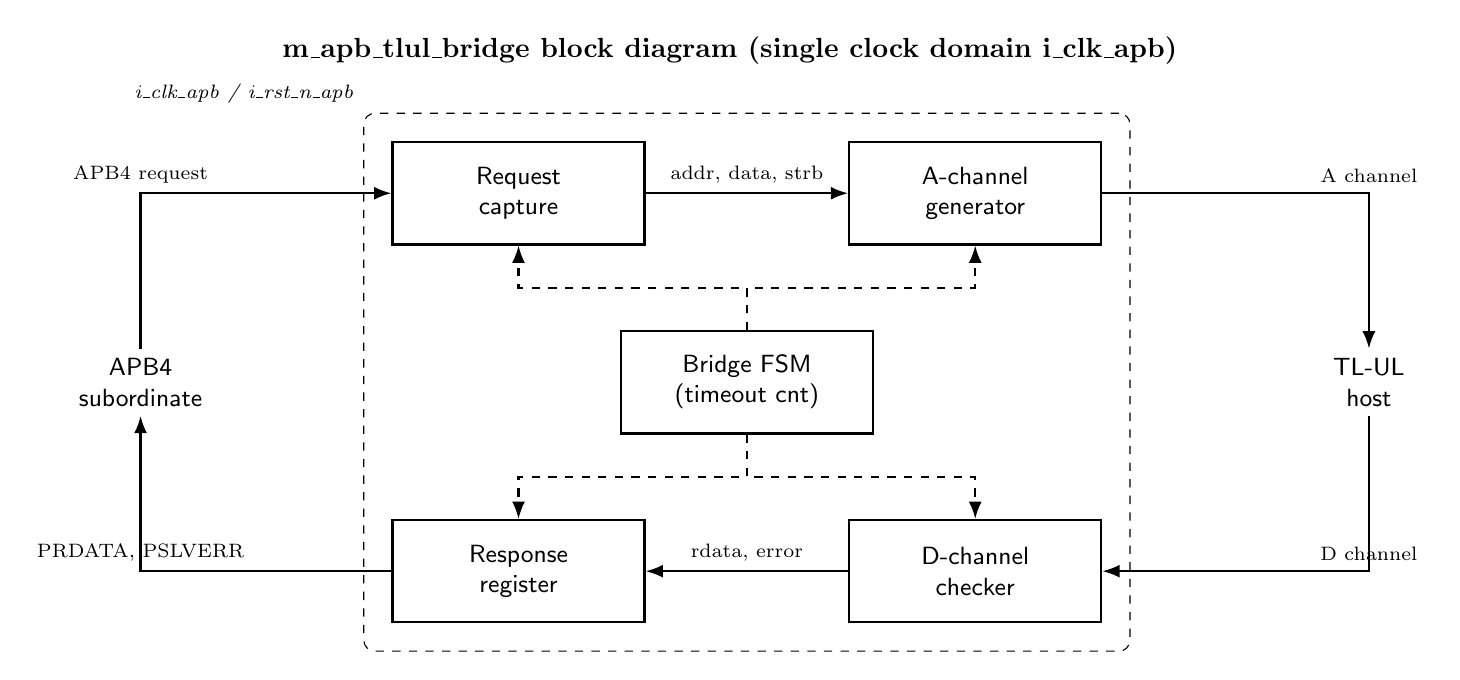
\begin{tikzpicture}[font=\sffamily\small,
  blk/.style={draw,thick,minimum width=3.2cm,minimum height=1.3cm,align=center,fill=white},
  mem/.style={blk,double,double distance=1.5pt},
  clk/.style={blk,rounded corners=6pt},
  io/.style={align=center,minimum width=1.6cm,minimum height=0.8cm},
  data/.style={-{Latex[length=2.2mm]},thick},
  ctrl/.style={-{Latex[length=2.2mm]},thick,dashed},
  clock/.style={-{Latex[length=2.2mm]},thick,dotted}]
\node[io] (io_apb) at (0.00,-2.40) {APB4\\ subordinate};
\node[blk] (cap) at (4.80,0.00) {Request\\ capture};
\node[blk] (agen) at (10.60,0.00) {A-channel\\ generator};
\node[io] (io_tl) at (15.60,-2.40) {TL-UL\\ host};
\node[blk] (fsm) at (7.70,-2.40) {Bridge FSM\\ (timeout cnt)};
\node[blk] (rsp) at (4.80,-4.80) {Response\\ register};
\node[blk] (rchk) at (10.60,-4.80) {D-channel\\ checker};
\draw[data] (io_apb.north) |- node[midway,above,font=\scriptsize,align=center]{APB4 request} (cap.west);
\draw[data] (cap.east) -| ($(cap.east)!.5!(agen.west)$) |- node[midway,above,font=\scriptsize,align=center]{addr, data, strb} (agen.west);
\draw[data] (agen.east) -| node[midway,above,font=\scriptsize,align=center]{A channel} (io_tl.north);
\draw[data] (io_tl.south) |- node[midway,above,font=\scriptsize,align=center]{D channel} (rchk.east);
\draw[data] (rchk.west) -| ($(rchk.west)!.5!(rsp.east)$) |- node[midway,above,font=\scriptsize,align=center]{rdata, error} (rsp.east);
\draw[data] (rsp.west) -| node[midway,above,font=\scriptsize,align=center]{PRDATA, PSLVERR} (io_apb.south);
\draw[ctrl] (fsm.north) |- ($(fsm.north)!.5!(cap.south)$) -| (cap.south);
\draw[ctrl] (fsm.north) |- ($(fsm.north)!.5!(agen.south)$) -| (agen.south);
\draw[ctrl] (fsm.south) |- ($(fsm.south)!.5!(rsp.north)$) -| (rsp.north);
\draw[ctrl] (fsm.south) |- ($(fsm.south)!.5!(rchk.north)$) -| (rchk.north);
\begin{scope}[on background layer]
\node[draw,dashed,rounded corners=4pt,inner sep=10pt,fit=(cap)(agen)(fsm)(rsp)(rchk),label={[font=\scriptsize\itshape]north west:i\_clk\_apb / i\_rst\_n\_apb}] (g0) {};
\end{scope}
\node[font=\bfseries,anchor=south] at (current bounding box.north) {m\_apb\_tlul\_bridge block diagram (single clock domain i\_clk\_apb)};
\end{tikzpicture}
\end{document}
